\documentclass[a4paper]{article}
\usepackage[english]{babel}
\usepackage[utf8]{inputenc}

% mathermatics
\usepackage{amssymb} % useful math symbols
\usepackage{mathrsfs,amsmath} % more useful math (mathrsfs for Fourier F)
\usepackage{bm} % for nice matrices in ISO standard formatting

% graphics
\usepackage{graphicx}
\usepackage{float}    % for more accurate graphics placement
\usepackage{fancyhdr} % for top header

% references
\usepackage{hyperref} % needed by cleveref, also provides clickable links
\usepackage{cleveref} % needed by autonum
\usepackage{autonum} % only add numbers to referenced equations

% formatting
\usepackage{enumitem} % provides easy change of labels in enumerate environment
\usepackage[top=3cm, bottom=4cm, width=17cm]{geometry} % for smaller page margins
\usepackage{multirow}

% colors
\usepackage{xcolor}

% coding
% 
% uncomment this after you have completed the required installation
% see https://github.com/gpoore/minted for info

\usepackage{minted} 
\definecolor{codeBgColor}{RGB}{240,240,240}




% very simple alias, \ex{} becomes the same as \subsubsection*{}
% TIP: remove the * in the line below if you want it numbered
\newcommand{\ex}[1]{\subsubsection*{#1}}




%Begining of the document
\begin{document}

\pagestyle{fancy} % use pagestyle with simple header (from fancyhdr)

%\pagenumbering{gobble} % uncomment to remove pagenumbering (in case of single page document)
\fancyhead[L]{TMA4135 Matematikk 4D}
\fancyhead[C]{\textbf{Exercise 11}}
\fancyhead[R]{Otto Lote (748704)}
\fancyfoot{}

\ex{1}


\begin{enumerate}[label=\alph*)]
    \item We use the following script to find the DFT of the discrete time series

            \begin{minted}
                [
                    linenos,                % line numbers
                    bgcolor=codeBgColor     % background color, remove for none
                ]
                {matlab} 
% Discrete time series x
x = [0, 2, 3, 7];

% Fast fourier transform of x, then take the real part
y = fft(x);
r = real(y);

plot(r);
            \end{minted}
    \item This results in the following plot
        \begin{figure}[H]
            \centering
            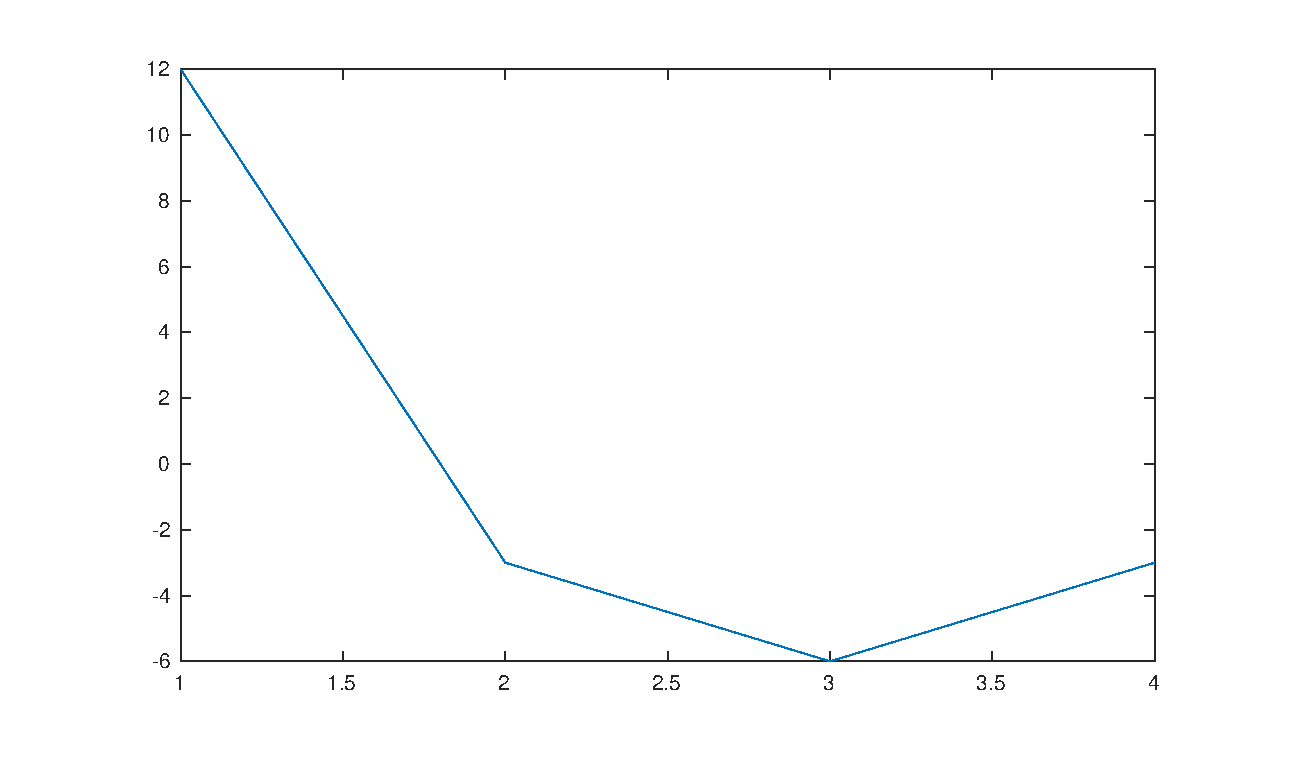
\includegraphics[width=0.7\textwidth]{task1.eps}
            \caption{Matlab plot of the real part of the \texttt{fft} of the
                discrete time series}
        \end{figure}
\end{enumerate}

\newpage
\ex{2}

We have the system of equations
\begin{align}
    5x_1 + x_2 + 2x_3 &= 19 \\
    x_1 + 4x_2 - 2x_3 &= -2 \\
    2x_1 + 3x_2 + 8x_3 &= 39 \\
\end{align}
\begin{align}
    \intertext{Which can be rewritten to}
    x_1 &= - 0.200x_2 - 0.400x_3 + 3.800  \\
    x_2 &= - 0.250x_1 + 0.500x_3 - 0.500 \\
    x_3 &= - 0.250x_1 - 0.375x_2 + 4.875 \\
\end{align}



\begin{enumerate}[label=\alph*)]
    \item 
        \begin{align}
            \intertext{We can write the system on the form \(\bm{A}\bm{x} =
                \bm{b}\) using the matrices \(\bm{A} = \bm{I} + \bm{L} +
                \bm{U}\) where}
            \bm{U} &=
            \begin{bmatrix}
                0 & 0.2 & 0.4 \\
                0 & 0 & -0.5 \\
                0 & 0 & 0 \\
            \end{bmatrix}, \quad
            \bm{L} =
            \begin{bmatrix}
                0 & 0 & 0 \\
                0.25 & 0 & 0 \\
                0.25 & 0.375 & 0 \\
            \end{bmatrix} \\
            \bm{A} &= \bm{I} + \bm{L} + \bm{U} =
            \begin{bmatrix}
                1 & 0.2 & 0.4 \\
                0.25 & 1 & -0.5 \\
                0.25 & 0.375 & 1 \\
            \end{bmatrix} 
            \text{ and }
            \bm{b} = 
                \begin{bmatrix}
                    3.8 \\
                    -0.5 \\
                    4.875 \\
                \end{bmatrix}
        \end{align}

        We know the Gauss-Seidel iteration converges for \(||\bm{C}|| < 1\)
            where the iteration matrix \(\bm{C} = -(\bm{I}+\bm{L})^{-1}\bm{U}\)

        Calculating the \(\bm{C}\) matrix we get \(\bm{C} = [0, 0.125,
            0.2]^T\), which means the Gauss-Seidel iteration converges as all values of \(\bm{C}\) are less than 1.

        The Jacobi iteration matrix is given by \(\bm{I} - \bm{A}\) and the
            iteration converges if and only if this matrix has a spectral
            radius of less than 1. We can find the spectral radius of this
            matrix by using the matlab command \texttt{max(abs(eig(eye(3) -
            A)))} which outputs \texttt{0.2640}. This means the Jacobi
            iteration converges.

    \item 
        \begin{align}
        \end{align}
\end{enumerate}




%% uncomment this if you need references. Edit the .bbl file with your references
%% and use "\cite{bibitem-label}" to cite
%\bibliography{template}

\end{document}

